%%%
%%% BACHELOR'S THESIS TEMPLATE - ENGLISH
%%%
%%%  * the master file
%%%
%%%  This template requites compilation by the sequence
%%%    latex -> bibtex -> latex (2x) -> dvips -> ps2pdf
%%%  cslatex can be used instead of latex
%%%  pdflatex or pdfcslatex can be used if certain parts are adjusted
%%%
%%%  AUTHORS:  Martin Mares (mares@kam.mff.cuni.cz)
%%%            Arnost Komarek (komarek@karlin.mff.cuni.cz), 2011
%%%            Michal Kulich (kulich@karlin.mff.cuni.cz), 2013
%%%
%%%  LAST UPDATED: 20130318
%%%
%%%  ===========================================================================

%%%%% Single page layout:
%%%%% ----------------------------------------------------
\documentclass[12pt, a4paper]{report}
\setlength\textwidth{145mm}
\setlength\textheight{247mm}
\setlength\oddsidemargin{15mm}
\setlength\evensidemargin{15mm}
\setlength\topmargin{0mm}
\setlength\headsep{0mm}
\setlength\headheight{0mm}
\let\openright=\clearpage


%%%%% Double page layout
%%%%% ----------------------------------------------------
% \documentclass[12pt, a4paper, twoside, openright]{report}
% \setlength\textwidth{145mm}
% \setlength\textheight{247mm}
% \setlength\oddsidemargin{15mm}
% \setlength\evensidemargin{0mm}
% \setlength\topmargin{0mm}
% \setlength\headsep{0mm}
% \setlength\headheight{0mm}
% \let\openright=\cleardoublepage



%%% Additional useful packages
%%% ----------------------------------------------------------------
\usepackage{amsmath}
\usepackage{amsfonts}
\usepackage{amsthm}
\usepackage{bm}
\usepackage{graphicx}
\usepackage{psfrag}
\usepackage{fancyvrb}
\usepackage[round]{natbib}
\usepackage{bbding}
\usepackage{dcolumn}
\usepackage{booktabs}
\usepackage{paralist}
\usepackage{indentfirst}
\usepackage[nottoc]{tocbibind}
\usepackage{minted}

\usepackage[latin1]{inputenc}
\usepackage[unicode]{hyperref}
\hypersetup{pdftitle=Thesis Title,
            pdfauthor=Name Surname,
            ps2pdf,
            pdfstartview=FitH,
            pdfpagemode=UseOutlines,
            pdfnewwindow,
            breaklinks
		}
\hypersetup{
  colorlinks   = true, %Colours links instead of ugly boxes
  urlcolor     = blue, %Colour for external hyperlinks
  linkcolor    = blue, %Colour of internal links
  citecolor    = red   %Colour of citations
		}



%%% -------------------------------------
\newcommand{\FIGDIR}{./Imagenes}    %%% directory containing figures
\newcommand{\CHAPDIR}{./Capitulos}  %%% directory containing chapters
\renewcommand{\chaptername}{Cap�tulo}
\renewcommand{\appendixname}{Ap�ndice}
\renewcommand{\contentsname}{Lista de contenidos}
\renewcommand{\figurename}{Figura}
\renewcommand{\listfigurename}{Lista de figuras}
\renewcommand{\tablename}{Tabla}
\renewcommand{\listtablename}{Lista de tablas}
\renewcommand{\bibname}{Bibliograf�a}



\theoremstyle{plain}
\newtheorem{veta}{Theorem}
\newtheorem{lemma}[veta]{Lemma}
\newtheorem{tvrz}[veta]{Proposition}

\theoremstyle{plain}
\newtheorem{definice}{Definition}

\theoremstyle{remark}
\newtheorem*{dusl}{Corollary}
\newtheorem*{pozn}{Note}
\newtheorem*{prikl}{Example}


\newenvironment{dukaz}{
  \par\medskip\noindent
  \textit{Proof}.
}{
\newline
\rightline{\SquareCastShadowBottomRight}
}


\bibliographystyle{plainnat}     %% Author (year) style
%\bibliographystyle{unsrt}        %% [number] style


%%%%% ------------------------------------------------------------
\DefineVerbatimEnvironment{PCinout}{Verbatim}{fontsize=\small, frame=single}



\newcommand{\R}{\mathbb{R}}
\newcommand{\N}{\mathbb{N}}

\DeclareMathOperator{\pr}{\textsf{P}}
\DeclareMathOperator{\E}{\textsf{E}\,}
\DeclareMathOperator{\var}{\textrm{var}}
\DeclareMathOperator{\sd}{\textrm{sd}}


\newcommand{\T}[1]{#1^\top}

\newcommand{\goto}{\rightarrow}
\newcommand{\gotop}{\stackrel{P}{\longrightarrow}}
\newcommand{\maon}[1]{o(n^{#1})}
\newcommand{\abs}[1]{\left|{#1}\right|}
\newcommand{\dint}{\int_0^\tau\!\!\int_0^\tau}
\newcommand{\isqr}[1]{\frac{1}{\sqrt{#1}}}

\newcommand{\pulrad}[1]{\raisebox{1.5ex}[0pt]{#1}}
\newcommand{\mc}[1]{\multicolumn{1}{c}{#1}}



%%%%% Main document
%%%%% ---------------------

\begin{document}


%%%
%%% BACHELOR'S THESIS TEMPLATE - ENGLISH
%%%
%%%  * the title page and front matter
%%%
%%%  AUTHORS:  Martin Mares (mares@kam.mff.cuni.cz)
%%%            Arnost Komarek (komarek@karlin.mff.cuni.cz), 2011
%%%            Michal Kulich (kulich@karlin.mff.cuni.cz), 2013
%%%
%%%  LAST UPDATED: 20130318
%%%
%%%  ===========================================================================

\pagestyle{empty}
\begin{center}

{\large Universidad Complutense de Madrid}

\medskip
{\large Facultad de Inform�tica}

\vfill
{\bfseries\Large TRABAJO DE FIN DE GRADO}

\vfill
\centerline{\mbox{\includegraphics[width=60mm]{\FIGDIR/ucm_icono.eps}}}

\vfill
\vspace{5mm}

{\LARGE Daniel Gamo Alonso}

\vspace{15mm}

% Title in English according to the official assignment
{\LARGE\bfseries Generaci�n de descripciones de im�genes mediante \textit{Deep Learning}}

\vfill

Doble Grado en Ingenier�a Inform�tica y Matem�ticase
%%% department that confirmed the assignment of the thesis
%%% according to the Internal Structure of MFF UK in English
%%% see http://www.mff.cuni.cz/toUTF8.en/fakulta/struktura/sekcem.htm
% Department of Algebra
% Department of Mathematics Education
% Department of Mathematical Analysis
% Department of Numerical Mathematics
% Department of Probability and Mathematical Statistics
% Mathematical Institute of Charles University

\vfill

\begin{tabular}{rl}

\noalign{\vspace{2mm}}
Directores: & Alberto D�az Esteban, Gonzalo M�ndez\\

\end{tabular}

\vfill

% Fill the year
5 de julio de 2017

\end{center}


%%% At this place, the printed version includes a page containing the
%%% photocopy of the official signed "Bachelor thesis assignment".
%%% This should not be included in the electronic version.


%%% Acknowledgments
\newpage
\openright

\noindent
TODO - Agradecimientos

\newpage
%%% Czech and English abstracts

\vbox to 0.5\vsize{
\setlength\parindent{0mm}
\setlength\parskip{5mm}

\begin{center}
Resumen
\end{center}

El objetivo de este trabajo es construir un sistema basado en \textit{deep learning}
con el prop�sito de generar descripciones textuales a partir de las im�genes que se
suministren como entrada. Para ello se utilizar�n distintas t�cnicas relacionadas
con la visi�n artificial y el procesamiento del lenguaje natural como redes
neuronales y otras metodolog�as basadas en modelos
estad�sticos para, a partir de los elementos presentes en las
im�genes, predecir y generar descripciones coherentes con su contenido. Entre
las posibles aplicaciones podr�a estar el facilitar la accesibilidad a contenido
en forma de imagen a  usuarios con alg�n tipo de discapacidad visual.
\\
\\
\textbf{Palabras clave:} \textit{deep learning}, red neuronal, descripci�n de im�genes.


TODO: ENGLISH

\vss}

%%% A page containing the automatically generated contents of the
%%% bachelor thesis. For a mathematical thesis it is allowed to
%%% place the list of tables and abbreviations at the beginning
%%% of the thesis instead of at the end.
\newpage
\openright

\pagestyle{plain}
\setcounter{page}{1}

\tableofcontents


%%%
%%% BACHELOR'S THESIS TEMPLATE - ENGLISH
%%%
%%%  * the first chapter
%%%
%%%  AUTHORS:  Arnost Komarek (komarek@karlin.mff.cuni.cz), 2011
%%%            Michal Kulich (kulich@karlin.mff.cuni.cz), 2013
%%%
%%%  LAST UPDATED: 20130318
%%%

\chapter{Introducci�n}

A menudo se dice que una imagen vale m�s que mil palabras, y este dicho no podr�a
ser m�s acertado. Los humanos nos apoyamos en el sentido de la vista para gran
parte de las tareas que realizamos en nuestra vida cotidiana. Esta importancia
motiva el contenido de nuestro trabajo, en el que pretendemos construir un modelo
usando t�cnicas de \textit{deep learning} (con las que se han conseguido grandes
avances en los �ltimos a�os, e incluso meses, dentro de este campo) para estudiar la tarea
de analizar y extraer datos de las im�genes. Sin embargo, la importancia de la visi�n
para los humanos no se basa exclusivamente en reconocer objetos, que es la primera
aproximaci�n que se hace en este sentido, sino que tambi�n contamos con esa poderosa
herramienta que es el lenguaje, y que nos permite no solo reconocer, sino describir
lo que vemos. Esta idea de conexi�n entre la vista y el lenguaje es la que constituye
el grueso de este trabajo, y nuestro objetivo va a ser estudiar y construir un modelo
que relacione el contenido de una im�gen con una descripci�n textual de la misma.

En este proceso de an�lisis y descripci�n hay que tener diversos factores en cuenta.
Para empezar, hay que definir que vamos a entender por descripciones. Esta tarea
es dif�cil debido al amplio significado que tiene la tarea de describir; no est� claro c�mo de larga puede
ser la descripci�n, si debe centrarse en todos los detalles o dar una "idea general"
del contenido de la im�gen, etc. Todas estas razones convierten la tarea de la
descripci�n de im�genes en algo mucho m�s complejo,
alejado del planteamiento algo m�s sencillo (que no trivial) de extraer elementos de las im�genes
y organizarlos en una frase bien estructurada.

%%%%% ===============================================================================
\section{Objetivos}
Nuestro objetivo principal en este trabajo es construir un sistema que sea capaz de
relacionar el contenido de una imagen con una descripci�n textual que se acerque a
la que dar�a una persona. Para ello vamos a estudiar, desde el enfoque del \textit{deep learning},
las diferentes t�cnicas y modelos existentes para el an�lisis de im�genes y la descripci�n de su contenido.
Destacamos dos conceptos claves para el desarrollo de nuestro trabajo, que son
las redes neuronales recurrentes (\textit{Recurrent Neural Network}, RNN) y las redes
neuronales convolucionales (\textit{Convolutional Neural Network}, CNN), que han probado su eficacia
en las tareas relacionadas con procesamiento del lenguaje natural y an�lisis de im�genes, respectivamente.
Hablaremos en profundidad sobre ello en los cap�tulos 2 y 3 de esta memoria.

Para esta tarea necesitamos analizar una gran cantidad de datos. Cuando se suministra a una m�quina, una imagen
queda representada como una matriz de p�xeles y una sentencia (descripci�n) como una lista de palabras
(\textit{tokens}). Cada una de estas unidades no da informaci�n por si misma; necesita del resto para
conformar una unidad con sentido. Adem�s, para inferir las reglas que permitan detectar las relaciones
entre los distintos elementos (entre elementos de la imagen, entre elementos de la sentencia y entre
elementos de la imagen con su correspondiente sentencia) necesitamos un gran n�mero de im�genes y
de sentencias, con lo que la capacidad de computaci�n necesaria para llevarlo a cabo es inmensa.
En nuestro caso, contamos con una tarjeta gr�fica donada por NVIDIA que ser� clave en la realizaci�n
de todos los c�lculos involucrados en un tiempo aceptable.

%%%%% ===============================================================================
\section{�Qu� es una descripci�n?}
Ya hemos comentado la importancia que tiene definir correctamente lo que nuestro modelo
va a entender por una descripci�n. Tenemos un modelo generativo, que necesita descripciones
en el entrenamiento con un formato m�s o menos similar para producir buenos resultados.

Seg�n la RAE, describir se define como:
\begin{enumerate}
\item Representar o detallar el aspecto de alguien o algo por medio del lenguaje.
\item Moverse a lo largo de una l�nea.
\item Definir imperfectamente algo, no por sus cualidades esenciales, sino dando una idea general de sus partes o propiedades.
\item Delinear, dibujar, pintar algo, represent�ndolo de modo que se d� perfecta idea de ello.
\end{enumerate}

En el proceso de descripci�n de una escena, si nos atenemos a la tercera acepci�n,
no se hace un an�lisis detallado de todos los objetos y acciones que se reflejan
en ella, sino que se resume la informaci�n, y se tiende a describir los elementos
que m�s llaman nuestra atenci�n. Ya sea por su importancia o tama�o en la escena,
por la impresi�n subjetiva que nos causan o por el contexto en el que sucede la escena y
que los dota de mayor o menor relevancia.
Pensemos por ejemplo en una imagen de una persona con el cielo de fondo;
un humano destacar�a a la persona que aparece en ella y dar�a menos importancia a otras cosas
como el cielo que aparece detr�s de la imagen (no es algo que llame la atenci�n,
siempre esta ah�), mientras que una m�quina podr�a centrar su
atenci�n en ese cielo que aparece de fondo (por ejemplo, porque ocupa un porcentaje
de la imagen m�s alto que la persona).

En los \textit{datasets} que vamos a utilizar, cada imagen va acompa�ada de cinco
frases con una longitud media de ///CALCULAR CON EL CODIGO. La anotaci�n de im�genes
se ha realizado utilizando operarios humanos a trav�s de la plataforma Amazon Mechanical Turk. Se pidi� a
los trabajadores que describiesen el contenido de la imagen con una frase.
Se ha probado emp�ricamente que en esta colecci�n de datos se suele describir los
aspectos m�s relevantes de la imagen, con especial incapi� en descripci�n de personas,
sus acciones, interacciones con la gente o el entorno. [\citet{karpathy}].

\section{Problemas}
La tarea que nos proponemos presenta una seria de desaf�os m�s all� de la construcci�n
del modelo o de la capacidad de c�lculo de la que disponemos.

Cuesta decidir qu� es una buena descripci�n de una imagen y qu� no lo es, pues dos personas distintas podr�an
dar dos descripciones distintas de la misma imagen, ya sea por la importancia que dan a ciertos
elementos de la escena o por como describan el mismo elemento. Sin embargo, dos descripciones
distintas pueden ser igualmente v�lidas y esto pone de relieve la importancia de tener buenas m�tricas
para que el sistema sepa cu�ndo est� describiendo algo bien, cu�ndo est� describiendo algo mal, cuando
lo hace mejor y cuando lo hace peor. Desarrollaremos en el cap�tulo 4 con m�s detalle qu� m�tricas utilizamos,
cu�l es el razonamiento que hay detr�s de ellas y c�mo de fiables son.

Otro inconveniente que se nos presenta es la dificultad de obtener im�genes con buenas descripciones asociadas.
Aunque hay sitios como Flickr que contienen muchas im�genes con descripciones, a menudo estas �ltimas no dan
informaci�n fiable sobre el contenido de la imagen. Cuando subimos una fotograf�a, no solemos describir su
contenido, sino que adjuntamos texto sobre la situaci�n en la que se produce, las personas que nos acompa�an
o los sentimientos que nos evocan. Por esta raz�n, no es f�cil obtener autom�ticamente un \textit{dataset} lo bastante bueno
como para entrenar al sistema, y precisamos de trabajo humano para acompa�ar las im�genes (o partes concretas de las im�genes)
de descripciones adecuadas. En este sentido, muchos de los \textit{datasets} que se utilizan en este campo han requerido
del trabajo de muchas personas, principalmente utilizando la herramienta Amazon Mechanical Turk.
Adem�s, en relaci�n con lo que hemos expuesto en el p�rrafo anterior, necesitamos m�s
de una descripci�n por imagen para dar perspectiva a nuestro sistema sobre las diferentes formas de describir el mismo contenido.
Como en el caso de las m�tricas, la informaci�n acerca de los \textit{datasets} utilizados se desarrollar� en el cap�tulo ??.

Aunque tengamos un conjunto de pares imagen-descripci�n lo suficientemente grande y bueno para nuestra tarea, todav�a queda algo
que dificulta nuestra tarea, y es el poder asociar elementos de la descripci�n con zonas concretas de la imagen y no con toda ella.
En este sentido, se han publicado trabajos que cuentan con \textit{datasets} m�s completos en este sentido, como \textit{Visual Genome} [\citet{visualgenome}],
de manera que las relaciones entre lo descrito y su localizaci�n en la imagen son m�s f�ciles de aprender por el sistema.

%%%%% ===============================================================================
\section{Estructura del documento}
En el cap�tulo 1 hemos introducido el tema sobre el que trata esta memoria. El cap�tulo 2 consiste en un resumen sobre los trabajos m�s importantes
publicados acerca de an�lisis de im�genes, de sentencias y de relaci�n entre ambas. En el cap�tulo 3 describiremos nuestro modelo, y hablaremos sobre
la teor�a de \textit{deep learning} que hay detr�s del mismo. Adem�s describiremos la estructura y el funcionamiento de la redes neuronales que vamos
a implementar. En el cap�tulo 4 explicamos la metodolog�a que seguimos en nuestros experimentos y analizamos los datos y los resultados, compar�ndolos
con los de trabajos existentes. Se muestran adem�s ejemplos concretos de resultados que nuestro modelo a proporcionado. Por �ltimo, en el cap�tulo 5
exponemos las conclusiones del trabajo y planteamos lineas de trabajo futuras.
///////HASTA CAP 5?

%%%
%%% BACHELOR'S THESIS TEMPLATE - ENGLISH
%%%
%%%  * the second chapter
%%%
%%%  AUTHORS:  Arnost Komarek (komarek@karlin.mff.cuni.cz), 2011
%%%            Michal Kulich (kulich@karlin.mff.cuni.cz), 2013
%%%
%%%  LAST UPDATED: 20130318
%%%
%%%  ===========================================================================

\chapter{Trabajo relacionado}

%%%%% ===============================================================================
Tanto la tarea de an�lisis de im�genes como la de generaci�n de sentencias en lenguaje natural
mediante \textit{deep learning} est� en desarrollo constante, y cada mes aparece un nuevo art�culo
o tesis sobre este tema.

La idea de utilizar redes neuronales recurrentes para construir modelos relacionados
con el procesamiento del lenguaje natural est� muy presente en nuestro trabajo. En \citet{kombrink2011recurrent}
se propone un modelo que utiliza RNNs con este prop�sito, y analiza su comportamiento en esta tarea.
Existen numerosos estudios sobre la generaci�n de frases, donde nos interesan especialmente aquellos que
las construyen en base a unas etiquetas [\citet{2014neural}], m�s cercano a la idea de combinar
an�lisis de im�genes y sus descripciones (los elementos que aparecen en ellas se usan para generar las frases).

An�logamente, se ha probado que las redes neuronales convolucionales dan buenos resultados
cuando estamos tratando con datos en forma de imagen, como en \cite{2012imagenet}.
Sin embargo, tambi�n se plantea el problema de conseguir buenos tiempos de entrenamiento
en estas redes con tantos par�metros que ajustar. 

Para trabajar con las t�cnicas de \textit{deep learning}, han aparecido numerosas APIs
que automatizan gran parte de los c�lculos necesarios en la red. Entre ellas destacamos
Theano (la que usaremos en este proyecto) y TensorFlow, que cuenta con el apoyo de Google.

En el trabajo de \cite{matchwords} se explora la conexi�n entre im�genes (o regiones de im�genes) y palabras
mediante diferentes modelos, a�n sin utilizar t�cnicas de \textit{deep learning}, presentes en las publicaciones
m�s actuales.

Los trabajos que combinan ambos enfoques para generar descripciones de im�genes son m�s recientes,
Estos son los que nos interesan, y que vamos a tomar como base para construir nuestro propio modelo.
El elemento com�n entre todos ellos es que se basan en redes neuronales convolucionales para el an�lisis de im�genes
y redes neuronales recurrentes para la generaci�n de frases [\citet{karpathy2015deep, vinyals2015show}].
En el trabajo de \citet{karpathy2015deep} se trabaja con una modificaci�n de las RNNs tradicionales
(introduciendo la bidireccionalidad en la red) y de las CNNs, para que ambas trabajen bien en conjunto.

Tambi�n es importante destacar la importancia de contar con buenos \textit{datsets} y metodolog�as
definidas para la evaluaci�n de parejas imagen-frase. En el trabajo de Hodosh et al. \cite{hodosh2013framing} se
recopilan anotaciones de 8000 im�genes (5 para cada una de las im�genes) que deben describir las entidades y los eventos.
Como en el resto de \textit{datasets} que vamos a estudiar en este trabajo, las anotaciones se han obtenido mediante trabajadores
humanos con plataformas de \textit{crowdsourcing}. Este \textit{dataset} se denomina Flickr8k. Mencionamos el trabajo relacionado
con otro de los \textit{datsets} que vamos a utilizar: MSCOCO \citet{mscoco}.

%%%
%%% BACHELOR'S THESIS TEMPLATE - ENGLISH
%%%
%%%  * the third chapter
%%%
%%%  AUTHORS:  Arnost Komarek (komarek@karlin.mff.cuni.cz), 2011
%%%            Michal Kulich (kulich@karlin.mff.cuni.cz), 2013
%%%
%%%  LAST UPDATED: 20130318
%%%
%%%  ===========================================================================

\chapter{Descripci�n de im�genes mediante deep learning}

Notas para el cap�tulo:

->Machine learning background
->Deep learning background (CNN, RNN)
->Image-sentence ranking task (c�mo se asocian im�genes y descripciones)
      *Estructura del modelo
      *Ecuaciones
      *...
->Predict sentences using images (c�mo se predicen descripciones para las im�genes)
      *Estructura del modelo
      *Ecuaciones
      *...

En este cap�tulo, presentamos los conceptos m�s importantes de
deep learning que vamos a utilizar para construir nuestro modelo.
Tras ello, hablamos primero sobre las redes neuronales convolucionales,
c�mo funcionan y que caracer�sticas las hacen buenas para el tratamiento
de im�genes. En la secci�n (REF) estudiamos las redes neuronales recurrentes
que utilizamos en la vertiente de procesamiento del lenguaje natural
para la generaci�n de sentencias.

\section{Machine Learning}
Comenzamos hablando de machine learning, campo en el que tambi�n se ubica el deep
learning. El machine learning consiste en desarrollar sistemas que reciben unos ejemplos
de la tarea que deben realizar, y a partir de ellos inferir reglas que permitan
a la m�quina completar esas tareas autom�ticamente.

En un sistema de machine learning diferenciamos varios elementos importantes: la tarea
a realizar, una medida del rendimiento y la experiencia del aprendizaje.

Algunas de las principales tareas a aprender en machine learning son:
\begin{enumerate}
 \item \textbf{Clasificaci�n.} El sistema dispone de $k$ categor�as, de forma
 que cada entrada $x \in X$ se mapea a una de estas categor�as v�a una funci�n
 $f:\mathbb{R}\rightarrow\{1,...,k\}$. 
 \item \textbf{Regresi�n log�stica.} Dada una entrada, queremos obtener un valor num�rico
 para la entrada correspondiente. En este caso, cada entrada $x \in X$ se mapea a
 un valor real mediante una funci�n $f:X\rightarrow\mathbb{R}$. La principal
 diferencia con la clasificaci�n es el formato de la salida.
\end{enumerate}

Para cuantificar c�mo se comporta el sistema, necesitaremos una medida del rendimiento,
que ser� espec�fica para cada tarea.

Por �ltimo, y seg�n c�mo sea la experiencia de aprendizaje, hablaremos de aprendizaje supervisado
(el sistema es alimentado con ejemplos correctos acompa�ados de su etiqueta o valor
correspondiente) o no supervisado (el sistema es alimentado con ejemplos para que
aprenda su estructura).

\section{Deep Learning}

\subsection{Red Neuronal Feedforward}
La red neuronal feedforward, tambi�n denominada perceptr�n multicapa (multilayer perceptron, MLP por sus siglas
en ingl�s) constituye la base del deep learning. El objetivo es que el modelo aproxime
el valor de una funci�n $f*$. Para aproximar el valor de esta funci�n, buscamos 
(aprendemos) los valores �ptimos de los par�metros $\theta$ del sistema de manera que la funci�n
$f(x;\theta)$ sea una buena aproximaci�n de $f*$.

\subsection{Loss function}
Para qu� sirve, cuales se suelen utilizar


\subsection{Descenso de gradiente estoc�stico (SGD)}
Explicar algoritmo, variantes (en especial las que vamos a utilizar; adam, rmsprop,...)


\section{Dataset}
Para entrenar nuestro modelo utilizaremos datasets consistentes
en una lista de im�genes, cada una de ellas acompa�ada de 5 descripciones.
Los datasets que vamos a utilizar son Flickr8k [\citet{hodosh2013framing}],
MSCOCO [\citet{mscoco}] y Flickr30k [\citet{young2014image}]. En deep learning,
se suele tener una divisi�n de los datasets  en tres partes, cada una con un
prop�sito concreto:

\begin{enumerate}
\item \textbf{Training set.} Son los datos que se utilizan para entrenar
al modelo. En el entrenamiento, el sistema recibe estos ejemplos para ajustar
una serie de par�metros con el objetivo de mejorar los resultados en la tarea
concreta que se est� llevando a cabo.

\item \textbf{Validation set.} Al entrenar, el sistema tiende al sobreajuste
(\textit{overfitting}): los par�metros de la red se ajustan muy bien a los
ejemplos concretos con los que se la entrena, pero ante un dato de entrenamiento
diferente ofrece malos resultados. Para evitarlo, se suministran ejemplos al
sistema que no forman parte de los datos de entrenamiento. Se calcula la precisi�n
del sistema con datos de entrenamiento y estos �ltimos de validaci�n, con la
intenci�n de actualizar los par�metros tras el entrenamiento s�lo si dicha
actualizaci�n mejora tambi�n los resultados sobre los datos de validaci�n.

\item \textbf{Testing set.} Tras el entrenamiento, estos datos se utilizan
para observar la precisi�n final alcanzada por la red y poder cuantificar
los resultados tras el entrenamiento.
\end{enumerate}

Estos datasets consisten en 8000, , y 31000, respectivamente. Para ambos, tomamos
1000 im�genes para validaci�n, 1000 im�genes para pruebas y el resto para
entrenamiento, como se hace en \citet{karpathy}.

\section{Asociando im�genes y descripciones}
La tarea principal de nuestro trabajo consiste en dise�ar un modelo que, dada una 
imagen como entrada, sea capaz de generar (predecir) una sentencia que la describa.
Para que esto sea posible, necesitamos una manera de asociar im�genes y sentencias,
asignando una puntuaci�n a una pareja (imagen, sentencia) que indique lo relacionados
que est�n ambos datos. As�, una pareja en la que la imagen quede bien descrita por
la sentencia tendr� mayor puntuaci�n que una pareja en la que la imagen y su sentencia
tengan poca relaci�n entre s�.
El problema es que tanto una imagen como una sentencia son objetos de alta dimensi�n,
de manera que asociar unos con otros no es una tarea inmediata.

\subsection{Representaci�n de im�genes}
Para representar las im�genes, podemos hacerlo de dos formas: codificar cada imagen
como un vector (global image encoding) o codificar cada imagen como un conjunto de 
vectores (fragment-level image encoding). Para simplificar nuestro modelo y mantener
tiempos de entrenamiento admisibles, usaremos la primera aproximaci�n.

Para transformar nuestra imagen de entrada en su representaci�n vectorial utilizaremos
una red neuronal convolucional, que toma la imagen $I$ (matriz de tama�o $Height * Weight * Depth$)
y aplica una serie de transformaciones hasta convertirla en un vector $v$. Representamos
esta transformaci�n mediante una funci�n $CNN_{\theta}$ (donde $\theta$ representa los
par�metros de la red. Un procedimiento habitual consiste en utilizar la CNN como un extractor
de caracter�sticas (\textit{feature extractor}) sobre las que se realiza el entrenamiento propiamente dicho.
Para ello, como se hace en numerosos trabajos [\citet{karpathy}], se preentrena una CNN con el 
reto de clasficaci�n de ImageNet\footnote{Disponible para su descarga en http://image-net.org/download},
consistente en una serie de im�genes y 1000 categor�as diferentes para su clasificaci�n. Tras ello, 
la �ltima capa de la CNN que implementa la clasificaci�n en s�. Todo este proceso da lugar a una CNN
con par�metros aprendidos (que denotaremos mediante $\theta_{0}$) que usaremos para realizar una transformaci�n
fija de la imagen.

\begin{equation}
  v = W[CNN_{\theta_{0}}(I)] + b
\end{equation} 

Entrenaremos el sistema para que aprenda los par�metros $W$ y $b$. (finetuning, backprop on CNN)



\subsection{Representaci�n de sentencias}


\section{Generaci�n de descripciones}

\section{Recurrent Neural Networks - RNNs}

A diferencia de las redes neuronales tradicionales, en las redes neuronales recurrentes
se considera que los datos de entrada (y salida) no son independientes entre s�.
Entre los principales usos de estas redes destacamos dos:

\begin{enumerate}
\item Clasificar sentencias de acuerdo a su probabilidad de aparecer en una situaci�n real,
d�ndonos una medida de su correcci�n sint�ctica y/o gram�tica.
\item Generar texto nuevo (original) tras entrenar el sistema con frases de prueba.
\end{enumerate}

Observamos la importancia de considerar dependencias entre las entradas y las salidas de la red:
en el caso de las frases, si queremos generar una nueva palabra, tendremos que tener en cuenta
la parte de la frase ya generada, pues esta influir� en el resto de la sentencia.

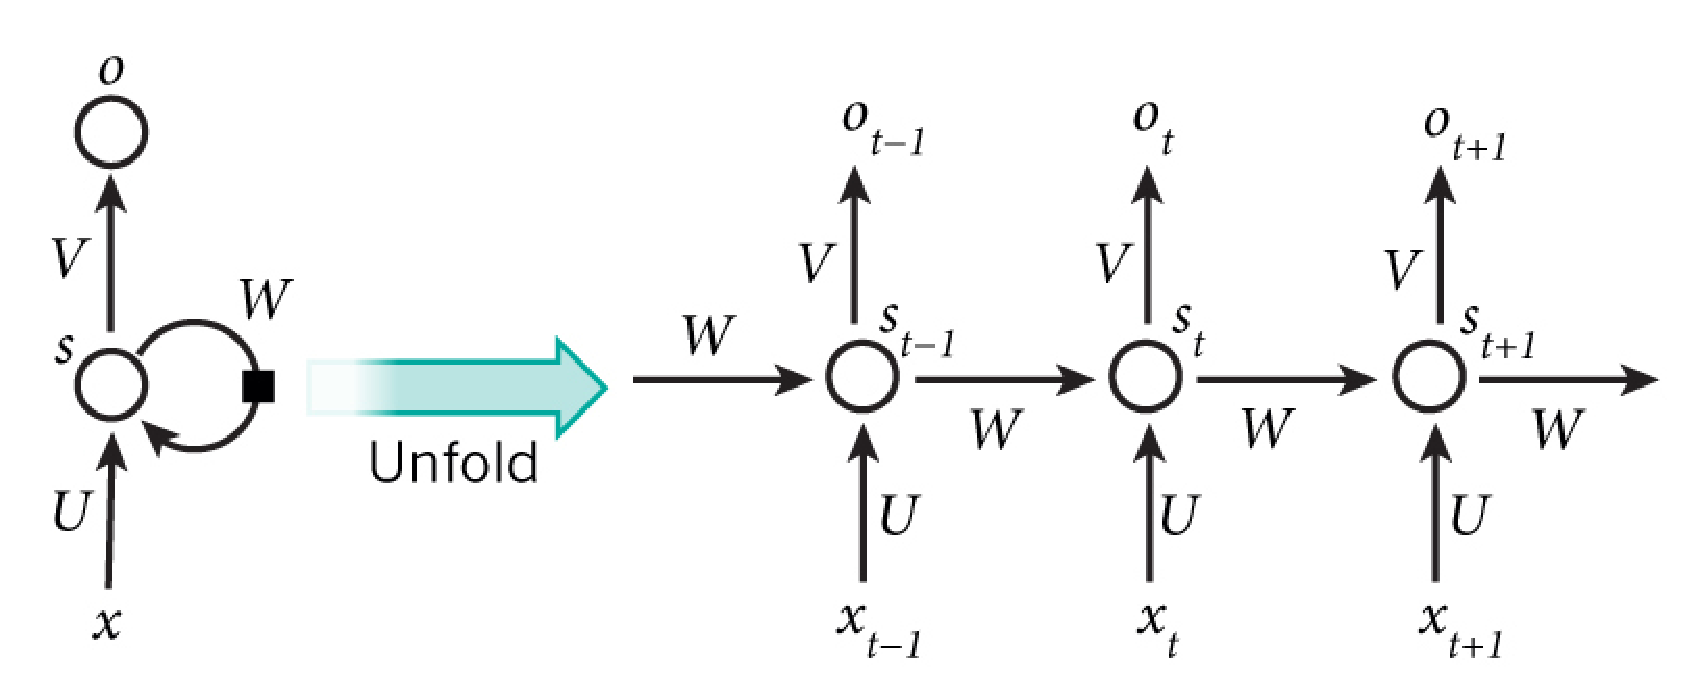
\includegraphics[width=\linewidth]{\FIGDIR/rnn.eps}

En este caso, $x_t$ representa la entrada de la red, $s_t$ el estado oculto y $o_t$
la salida en el paso $t$. En la figura vemos que el estado $s_t$ se calcula como
funci�n del estado anterior $s_{t-1}$, la entrada en el paso actual $x_t$.
La red posee "memoria" en el sentido en que los estados anteriores condicionan
el estado actual. Sin embargo, esta memoria no se mantiene durante muchas fases.
Existe un tipo concreto de RNN, las conocidas como \textit{long short-term memory}
(LSTM) que favorece la persistencia de los datos de los estados anteriores durante
un n�mero de mayor de fases, lo que las hace especialmente indicadas para comprensi�n
de lenguaje natural, an�lisis de textos manuscritos y reconocimiento de voz.

\section{Convolutional Neural Networks - CNNs}

Las redes neuronales convolucionales se utilizan en tareas como la clasificaci�n y reconocmiento de im�genes.

%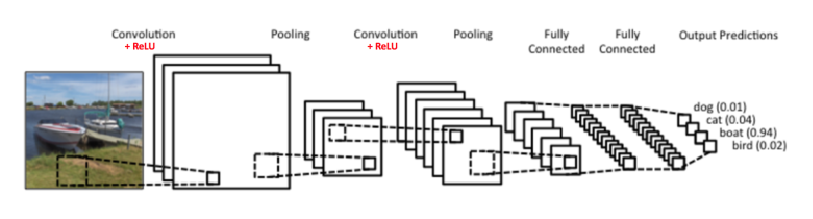
\includegraphics[width=\linewidth]{\FIGDIR/cnn.eps}

Podemos ver que el modelo asigna la mayor probabilidad a "barco" de entre las cuatro
categor�as existentes. En el modelo de la figura observamos cuatro operaciones en la red:

\begin{itemize}
\item \textbf{Convoluci�n.} El principal objetivo de la operaci�n de convoluci�n
es extraer caracter�sticas de una imagen.La convoluci�n preserva la relaci�n
espacial entre los pixels de la imagen usando peque�os cuadros como datos de entrada.

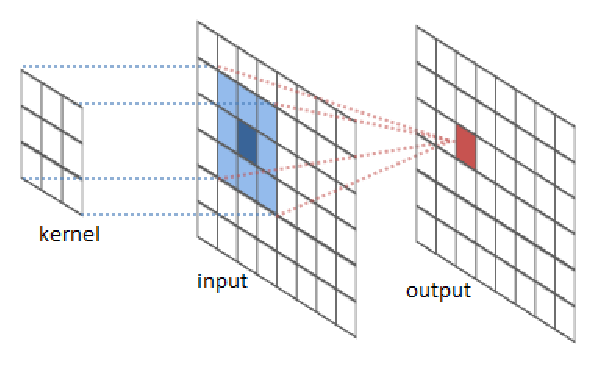
\includegraphics[width=\linewidth]{\FIGDIR/convolution.eps}

Consideramos una imagen como una matriz bidimensional de p�xeles (input), y otra
 matriz (\textit{kernel} o filtro), normalmente de tama�o $3x3$ que "recorre" la
 imagen de entrada. Con los valores del kernel y la porci�n de imagen que cubre,
 se computa la convoluci�n y esto da como resultado otra imagen (mapa de activaci�n).

\item \textbf{No linealidad.} Se aplica una funci�n de activaci�n no lineal operando
sobre cada pixel del mapa de activaci�n. Aunque pueden usarse funciones como la
sigmoide, se ha probado que la funci�n ReLU (Rectified Linear Unit) da mejores
resultados en este tipo de redes neuronales [REF].

%
\includegraphics[width=\linewidth]{\FIGDIR/relu.eps}

\item \textbf{Pooling.} Se encarga de reducir el tama�o del mapa de activaci�n
conservando los elementos m�s importantes. El \textit{Pooling} puede ser de
distintos tipos: Max, Sum, Avg...

%
\includegraphics[width=\linewidth]{\FIGDIR/maxpool.eps}

En el caso del \textit{Max Pooling}, se define un espacio (por ejemplo una matriz
 $2x2$) y para cada bloque $2x2$ se coge el mayor valor de entre los 4 existentes.

La funci�n del \textit{Pooling} es reducir las im�genes y convertirlas en objetos
 m�s manejables por las siguientes capas de la red.

\item \textbf{Fully Connected Layer.} Tras la convoluci�n y el \textit{Pooling},
obtenemos caracter�sticas de alto nivel de la imagen de entrada. En esta fase, y
usando dichas caracter�sticas como entrada, clasificamos la imagen en una serie
de categor�as basadas en el \textit{dataset} de entrenamiento.


\includegraphics[width=\linewidth]{\FIGDIR/fullycon.eps}

\end{itemize}


%%% References
%%% References are sought in the database priklady_literatury.bib.
%%% Requires the compilation sequence latex->bibtex->latex->latex
\bibliography{bibliografia}

%%% List of figures
%\listoffigures

%%% List of tables
%\listoftables

%%%
%\chapter*{List of abbreviations}
%\addcontentsline{toc}{chapter}{List of abbreviations}

%%% The Appendix.
%\chapter*{Appendix}
%\addcontentsline{toc}{chapter}{Appendix}

\end{document}
